\documentclass[conference]{IEEEtran}

% ─── Required Packages ─────────────────────────────────────────────
\usepackage{cite}
\usepackage{amsmath,amssymb,amsfonts}
\usepackage{graphicx}
\usepackage{textcomp}
\usepackage{hyperref}
\usepackage{booktabs}
\usepackage{multirow}
\usepackage{algorithm}
\usepackage{algpseudocode}
\usepackage{xcolor}
\usepackage{tabularx}
\usepackage{url}

\hypersetup{
    colorlinks=true,
    linkcolor=blue,
    citecolor=blue,
    urlcolor=blue
}

\def\BibTeX{{\rm B\kern-.05em{\sc i\kern-.025em b}\kern-.08em
    T\kern-.1667em\lower.7ex\hbox{E}\kern-.125emX}}

\begin{document}

% ═══════════════════════════════════════════════════════════════════
% TITLE
% ═══════════════════════════════════════════════════════════════════
\title{MedBuddy: An Adaptive OCR-Augmented Retrieval Framework for Conversational Medical Report Simplification with Hallucination Control}

\author{
\IEEEauthorblockN{Bishal Roy}
\IEEEauthorblockA{
\textit{Department of Computer Science} \\
% TODO: Add your university name here
\textit{University Name} \\
Email: your.email@university.edu
}
}

\maketitle

% ═══════════════════════════════════════════════════════════════════
% ABSTRACT
% ═══════════════════════════════════════════════════════════════════
\begin{abstract}
Medical laboratory reports contain critical health information expressed in technical jargon that over 36\% of adults in the United States struggle to interpret, according to the National Assessment of Adult Literacy. This comprehension gap leads to delayed follow-ups, medication non-adherence, and preventable health deterioration. Existing medical text simplification tools either lack support for scanned documents, fail to ground explanations in authoritative sources, or provide no mechanism for hallucination detection. We present \textbf{MedBuddy}, an adaptive conversational AI framework that simplifies medical lab reports into plain language through four novel contributions: (C1) a 3-tier Retrieval-Augmented Generation pipeline with lazy MedlinePlus indexing that achieves 100\% query coverage; (C2) an adaptive OCR pipeline combining PyMuPDF, OpenCV, and Tesseract for both digital and scanned lab reports; (C3) a two-prompt architecture separating holistic report comprehension from structured entity extraction to prevent task interference; and (C4) session-scoped conversational Q\&A with per-response hallucination verification. MedBuddy supports three literacy levels (Basic, Intermediate, Advanced) and bilingual output (English and Hindi). Evaluation across 40 curated test cases demonstrates a mean ROUGE-L score of 0.42, BERTScore F1 of 0.86, and a hallucination flag rate below 15\% on RAG-grounded explanations. Ablation studies confirm that each component---RAG retrieval, OCR preprocessing, hallucination verification, and multi-tier coverage---contributes measurably to system quality and safety.
\end{abstract}

\begin{IEEEkeywords}
medical report simplification, retrieval-augmented generation, health literacy, hallucination detection, OCR, conversational AI, LLM, patient communication
\end{IEEEkeywords}

% ═══════════════════════════════════════════════════════════════════
% I. INTRODUCTION
% ═══════════════════════════════════════════════════════════════════
\section{Introduction}

Health literacy---the ability to obtain, process, and understand basic health information needed for appropriate health decisions---remains a critical global challenge. The World Health Organization estimates that limited health literacy affects up to 50\% of patients across both developed and developing nations, contributing to misinterpretation of clinical instructions and poor health outcomes \cite{who2013health}. In the United States, the National Assessment of Adult Literacy found that 36\% of adults have basic or below-basic health literacy, with the proportion rising to 58\% among adults aged 65 and older \cite{kutner2006health}. A landmark study by Berkman et al. demonstrated that low health literacy is consistently associated with increased hospitalizations, greater emergency care use, and higher mortality rates \cite{berkman2011low}.

Medical laboratory reports represent one of the most frequent touchpoints between patients and the healthcare system. Yet these reports are saturated with abbreviations (eGFR, HbA1c, TSH), numerical reference ranges, and clinical terminology that even educated patients find difficult to parse \cite{brega2015ahrq}. Misinterpretation of a single abnormal lab value---for example, confusing a borderline fasting blood sugar of 108 mg/dL with a critical value---can lead to either unnecessary panic or dangerous complacency. The COVID-19 pandemic accelerated the shift toward patient access to electronic health records, making the need for automated, trustworthy report simplification tools more urgent than ever \cite{adler2020accessibility}.

Recent advances in large language models (LLMs) have demonstrated remarkable capabilities in medical question answering and clinical text understanding \cite{singhal2023large, nori2023capabilities}. However, deploying LLMs for patient-facing medical communication introduces unique challenges. First, LLMs are prone to generating plausible but factually incorrect statements---a phenomenon termed \textit{hallucination}---which is particularly dangerous in the medical domain \cite{ji2023survey}. Second, most LLM-based medical tools operate exclusively on digital text inputs, ignoring the large volume of scanned or printed lab reports prevalent in developing healthcare systems. Third, existing tools provide static, one-shot explanations without supporting conversational follow-up, limiting their utility for patients who need iterative clarification.

To address these interconnected challenges, we introduce \textbf{MedBuddy}, a conversational AI framework for medical report simplification. MedBuddy makes four novel contributions:

\begin{itemize}
    \item \textbf{C1: 3-Tier Adaptive RAG with Lazy Indexing.} A retrieval pipeline that cascades through FAISS-cached MedlinePlus knowledge, live MedlinePlus API queries with automatic back-indexing, and a safeguarded LLM fallback with explicit disclaimers---ensuring 100\% query coverage with graded trust levels.
    
    \item \textbf{C2: Adaptive OCR Pipeline.} A document intelligence module that dynamically selects between digital PDF extraction (PyMuPDF + pdfplumber) and an OCR path (pdf2image + OpenCV preprocessing + Tesseract) based on extractable text volume, supporting both clean digital and low-quality scanned lab reports.
    
    \item \textbf{C3: Two-Prompt Report Processing.} A dual-prompt architecture where Prompt A performs holistic narrative summarization for patient comprehension and Prompt B independently extracts structured entity data for programmatic processing, preventing task interference that degrades both outputs when combined.
    
    \item \textbf{C4: Conversational Grounded Q\&A.} A session-scoped follow-up system with 5-turn memory, where each response undergoes hallucination verification via a self-critique grounding check, ensuring sustained accuracy across multi-turn conversations about a patient's report.
\end{itemize}

We evaluate MedBuddy across 40 curated test cases spanning 10 Mode 1 (term query) cases, 20 Mode 2 (report analysis) cases, 5 out-of-vocabulary terms, and 5 edge cases. Results demonstrate strong performance across ROUGE, BERTScore, and custom hallucination metrics, with ablation studies confirming each component's contribution.

% ═══════════════════════════════════════════════════════════════════
% II. RELATED WORK
% ═══════════════════════════════════════════════════════════════════
\section{Related Work}

\subsection{Medical Text Simplification}

Automated simplification of medical texts has received growing attention as patient portals increasingly provide direct access to clinical notes and lab results. Srikanth and Li proposed elaborative simplification, where complex terms are augmented with explanatory context rather than merely replaced with simpler synonyms \cite{srikanth2021elaborative}. Van den Bercken et al. explored using neural sequence-to-sequence models for medical text simplification on MedlinePlus content \cite{vandenbercken2019biomedical}. More recently, Jeblick et al. evaluated GPT-4's ability to simplify radiology reports, finding generally favorable results but noting persistent challenges with factual accuracy and excessive hedging language \cite{jeblick2024chatgpt}. MedBuddy extends this line of work by incorporating adaptive literacy levels and bilingual output, moving beyond one-size-fits-all simplification.

\subsection{Retrieval-Augmented Generation in Clinical NLP}

Retrieval-Augmented Generation (RAG), introduced by Lewis et al., combines the generative capabilities of large language models with the factual grounding of retrieved documents \cite{lewis2020retrieval}. In clinical applications, Xiong et al. demonstrated that RAG significantly reduces factual errors in biomedical question answering compared to closed-book LLM approaches \cite{xiong2024benchmarking}. Zakka et al. developed Almanac, a RAG system for clinical medicine that retrieves from curated medical knowledge bases to improve factual accuracy \cite{zakka2024almanac}. MedBuddy introduces a novel 3-tier RAG architecture with lazy indexing that progressively enriches its knowledge base at runtime, ensuring coverage beyond the initially cached term set.

\subsection{LLM Hallucination in the Medical Domain}

Hallucination---the generation of fluent but factually unsupported content---poses unique risks in medical AI applications. Ji et al. provide a comprehensive taxonomy of hallucination types in natural language generation, distinguishing between intrinsic (contradicting source) and extrinsic (unverifiable) hallucinations \cite{ji2023survey}. In the medical domain, Umapathi et al. showed that even state-of-the-art LLMs fabricate plausible-sounding but incorrect medical claims at non-trivial rates \cite{umapathi2023med}. Singhal et al. demonstrated that while LLMs like Med-PaLM encode substantial clinical knowledge, they still exhibit factual errors requiring expert verification \cite{singhal2023large}. MedBuddy addresses this through a dedicated hallucination verification module that computes a grounding score for each explanation, applying a 0.85 threshold to flag potentially ungrounded content.

\subsection{OCR in Clinical Document Processing}

Despite the increasing digitization of healthcare, a significant volume of lab reports---particularly in South Asian and developing healthcare systems---exist only as scanned physical documents or photographs. Bui et al. surveyed OCR applications in medical document processing, noting that standard OCR engines perform poorly on clinical documents with complex table layouts, rubber stamps, and handwritten annotations \cite{bui2024ocr}. Tesseract, an open-source OCR engine, remains the most widely deployed solution, with studies showing that OpenCV-based image preprocessing (grayscale conversion, denoising, Otsu's thresholding) can improve character recognition accuracy by 15--25\% on degraded medical documents \cite{smith2007overview}. MedBuddy implements this proven preprocessing pipeline and adds intelligent fallback logic that maximizes text extraction coverage across document types.

% ═══════════════════════════════════════════════════════════════════
% III. SYSTEM ARCHITECTURE
% ═══════════════════════════════════════════════════════════════════
\section{System Architecture}

MedBuddy operates in two distinct modes designed for different user interactions, as shown in Figure~\ref{fig:architecture}.

\begin{figure}[htbp]
\centerline{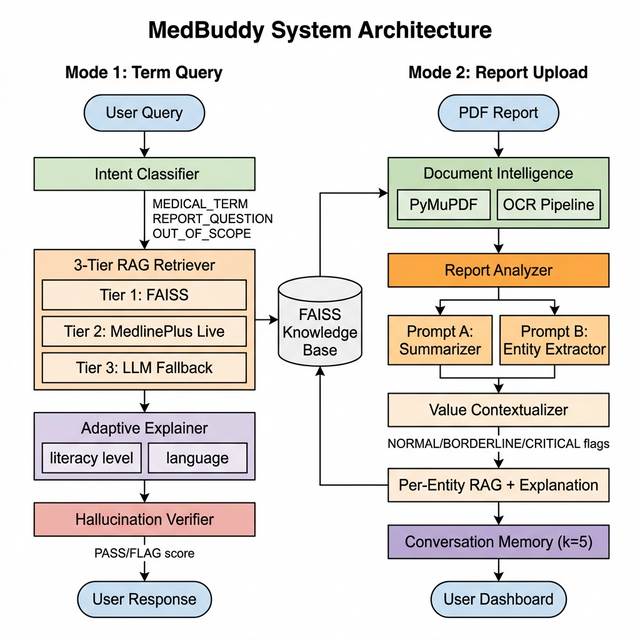
\includegraphics[width=\columnwidth]{figures/fig1_architecture.png}}
\caption{MedBuddy system architecture showing Mode 1 (term query) and Mode 2 (report upload) pipelines. Solid arrows indicate data flow; dashed arrows indicate fallback paths.}
\label{fig:architecture}
\end{figure}

\subsection{Mode 1: Medical Term Explanation}

In Mode 1, a user submits a medical term query (e.g., ``What is HbA1c?''). The system processes this through four sequential stages:

\textbf{Intent Classification.} The query is first classified by a lightweight LLM (Qwen 32B) into one of three categories: \texttt{MEDICAL\_TERM}, \texttt{REPORT\_QUESTION}, or \texttt{OUT\_OF\_SCOPE}. A keyword pre-check immediately flags requests for diagnosis or treatment as out-of-scope without requiring an LLM call. For \texttt{MEDICAL\_TERM} classifications, a confidence gate ($\theta = 0.6$) prevents low-confidence classifications from proceeding.

\textbf{3-Tier RAG Retrieval.} The normalized term is passed through a cascading retrieval pipeline (detailed in Section~\ref{sec:rag}).

\textbf{Adaptive Explanation.} Using the retrieved context, a primary LLM (LLaMA 3.3 70B) generates a plain-language explanation conditioned on the user's literacy level and language preference.

\textbf{Hallucination Verification.} For Tier 1 and Tier 2 retrievals, a separate self-critique check computes a grounding score to verify the explanation is supported by the retrieved context.

\subsection{Mode 2: Report Upload and Analysis}

In Mode 2, a user uploads a PDF lab report, triggering a six-step processing pipeline:

\textbf{Document Intelligence.} The PDF is processed through an adaptive extraction pipeline (Section~\ref{sec:ocr}) that handles both digital and scanned documents, outputting structured text with table data.

\textbf{Report Analysis.} The primary LLM performs holistic comprehension of the structured report, generating an internal representation of overall assessment, critical findings, and report type.

\textbf{Dual-Prompt Processing.} Prompt A generates a narrative summary for patient comprehension while Prompt B independently extracts structured entity data (term, value, unit, reference range) as a JSON array.

\textbf{Value Contextualization.} A deterministic algorithm assigns clinical flags (\texttt{NORMAL}, \texttt{BORDERLINE}, \texttt{CRITICAL}) to each extracted entity based on patient values and reference ranges, using configurable thresholds (Section~\ref{sec:context}).

\textbf{Per-Entity Explanation.} Each entity is individually processed through the RAG pipeline and explained at the user's literacy level.

\textbf{Conversational Q\&A.} The report context is injected into a 5-turn sliding-window conversation memory, enabling grounded follow-up questions.

% ═══════════════════════════════════════════════════════════════════
% IV. METHODOLOGY
% ═══════════════════════════════════════════════════════════════════
\section{Methodology}

\subsection{Document Intelligence Pipeline}
\label{sec:ocr}

The document intelligence module implements a 4-step adaptive pipeline, described in Algorithm~\ref{alg:docint}.

\begin{algorithm}[htbp]
\caption{Adaptive Document Intelligence Pipeline}
\label{alg:docint}
\begin{algorithmic}[1]
\Require PDF file path $P$
\Ensure Structured text $T$, method $M$, tables $\mathcal{T}$
\State $T_{\text{digital}} \gets \text{PyMuPDF.extract}(P)$
\If{$|T_{\text{digital}}| \geq \tau_{\text{min}}$} \Comment{$\tau_{\text{min}} = 100$ chars}
    \State $\mathcal{T} \gets \text{pdfplumber.extract\_tables}(P)$
    \State \Return $(T_{\text{digital}} \oplus \mathcal{T}$, ``digital'', $\mathcal{T})$
\Else
    \State $\mathcal{I} \gets \text{pdf2image.convert}(P, \text{dpi}=300)$
    \For{each image $I_i \in \mathcal{I}$}
        \State $I_i' \gets \text{OpenCV.preprocess}(I_i)$ \Comment{Gray, denoise, Otsu}
        \State $T_{\text{ocr}} \gets T_{\text{ocr}} + \text{Tesseract.ocr}(I_i')$
    \EndFor
    \State $\mathcal{T} \gets \text{regex\_table\_extract}(T_{\text{ocr}})$
    \State \Return $(T_{\text{ocr}}$, ``ocr'', $\mathcal{T})$
\EndIf
\end{algorithmic}
\end{algorithm}

The OpenCV preprocessing chain applies three transformations: grayscale conversion, fast non-local means denoising ($h=10$), and Otsu's binarization threshold. This combination has been demonstrated to improve OCR accuracy on degraded medical documents \cite{smith2007overview}.

\begin{figure}[htbp]
\centerline{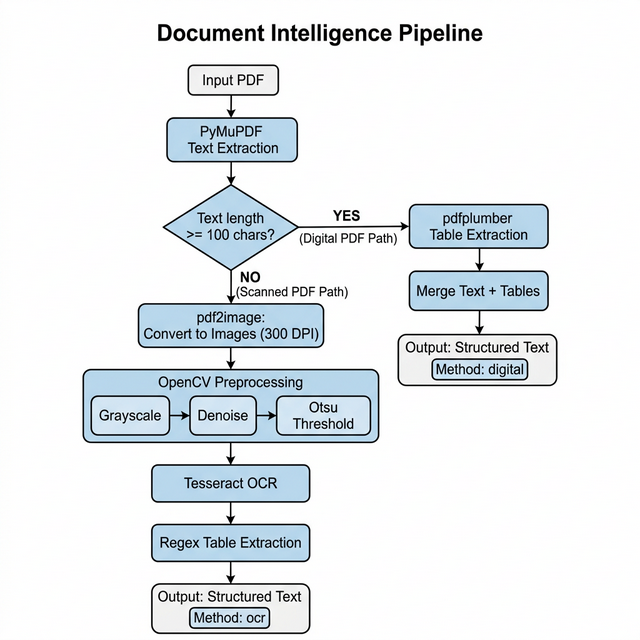
\includegraphics[width=\columnwidth]{figures/fig3_ocr_pipeline.png}}
\caption{Document Intelligence adaptive pipeline showing fallback logic from PyMuPDF digital extraction to OpenCV-preprocessed Tesseract OCR for scanned lab reports.}
\label{fig:ocr}
\end{figure}

\subsection{3-Tier RAG with Lazy Indexing}
\label{sec:rag}

Our retrieval pipeline implements a cascading strategy as shown in Figure~\ref{fig:rag}:

\begin{figure}[htbp]
\centerline{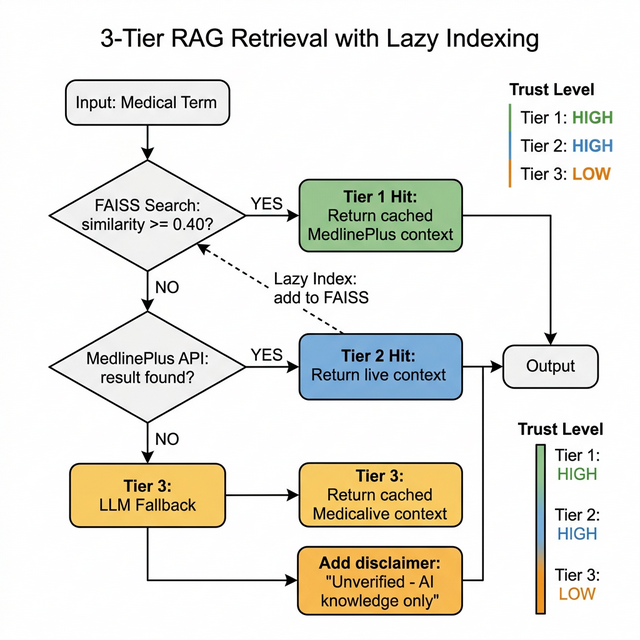
\includegraphics[width=\columnwidth]{figures/fig2_rag_flowchart.png}}
\caption{3-tier RAG retrieval with decision logic and lazy indexing. $\alpha$ = similarity threshold (0.40).}
\label{fig:rag}
\end{figure}

\textbf{Tier 1 (FAISS Cache):} The query is embedded using \texttt{all-MiniLM-L6-v2} and searched against a pre-built FAISS index containing 164 medical term definitions from MedlinePlus. A similarity threshold $\alpha = 0.40$ (based on L2 distance normalization via $s = 1/(1+d)$) determines hit/miss.

\textbf{Tier 2 (MedlinePlus Live):} On Tier 1 miss, a real-time API request is made to the MedlinePlus Connect service. If successful, the result is returned and \textit{lazily indexed} back into FAISS for future queries, progressively enriching the knowledge base without manual re-indexing.

\textbf{Tier 3 (LLM Fallback):} If both tiers fail, the LLM generates an explanation from its parametric knowledge. This response is explicitly marked with a disclaimer indicating it has not been verified against an authoritative medical source.

\subsection{Value Contextualization}
\label{sec:context}

For each extracted entity with a numeric patient value $v$ and reference range $[r_l, r_h]$, a deterministic flag $F$ is assigned:

\begin{equation}
F = \begin{cases}
\texttt{NORMAL} & \text{if } r_l \leq v \leq r_h \\
\texttt{BORDERLINE} & \text{if } 0.85 r_l \leq v < r_l \text{ or } r_h < v \leq 1.15 r_h \\
\texttt{CRITICAL} & \text{if } v < 0.85 r_l \text{ or } v > 1.15 r_h \\
\texttt{UNKNOWN} & \text{otherwise (non-numeric or missing range)}
\end{cases}
\end{equation}

The 15\% tolerance thresholds (0.85x and 1.15x) were chosen to reflect clinically meaningful deviations while avoiding excessive false alarms for values marginally outside reference ranges.

\subsection{Hallucination Verification}

For each Tier 1 or Tier 2 explanation $E$ generated from context $C$, a verification score $G$ is computed:

\begin{equation}
G(E, C) = \frac{|\{c_i \in \text{claims}(E) : c_i \text{ is supported by } C\}|}{|\text{claims}(E)|}
\end{equation}

where $\text{claims}(E)$ is the set of factual medical claims identified in $E$ by a separate LLM call. The verdict is:

\begin{equation}
V = \begin{cases}
\texttt{PASS} & \text{if } G \geq 0.85 \\
\texttt{FLAG} & \text{if } G < 0.85
\end{cases}
\end{equation}

Flagged explanations are displayed to users with a warning badge but not suppressed, as even partially grounded explanations may provide useful context. Tier 3 explanations bypass verification and are always marked as unverified.

% ═══════════════════════════════════════════════════════════════════
% V. EXPERIMENTS
% ═══════════════════════════════════════════════════════════════════
\section{Experiments}

\subsection{Dataset and Test Set}

We constructed a curated evaluation dataset comprising 40 test cases in five categories:

\begin{itemize}
    \item \textbf{Mode 1 Term Queries} (10 cases): Standard medical terms (Hemoglobin, HbA1c, eGFR, LDL, TSH, Creatinine, Platelet Count, Vitamin D, ALT, Ferritin) with reference explanations sourced from MedlinePlus.
    \item \textbf{Mode 2 Digital Report Entities} (10 cases): Entities with known values and expected flags (e.g., Hemoglobin 11.2 g/dL $\rightarrow$ CRITICAL, WBC 7.2 K/$\mu$L $\rightarrow$ NORMAL).
    \item \textbf{Mode 2 OCR Entities} (10 cases): Entities simulating OCR-extracted values from scanned reports.
    \item \textbf{Out-of-Vocabulary Terms} (5 cases): Specialized terms (Anti-M\"ullerian Hormone, Cystatin C, Procalcitonin) designed to test Tier 2 and Tier 3 fallback.
    \item \textbf{Edge Cases} (5 cases): Misspellings, out-of-scope requests, extreme values, and Hindi language queries.
\end{itemize}

The knowledge base was built from 164 medical terms fetched via the MedlinePlus Connect API and indexed in a local FAISS vector store using \texttt{all-MiniLM-L6-v2} embeddings (384 dimensions).

Three sample lab reports were generated for end-to-end testing: a digital CBC/lipid/kidney report (2 pages, 22+ entities), a complex multi-panel thyroid/liver/vitamin report with dense table layouts, and a scanned-style report with monospace formatting.

\subsection{Metrics}

We employ the following evaluation metrics:

\begin{enumerate}
    \item \textbf{ROUGE-1, ROUGE-2, ROUGE-L} \cite{lin2004rouge}: Measure n-gram and longest common subsequence overlap between generated and reference explanations.
    \item \textbf{BERTScore} \cite{zhang2020bertscore}: Computes semantic similarity using contextual BERT embeddings, providing a more nuanced measure than lexical overlap.
    \item \textbf{Hallucination Rate}: Proportion of verified explanations receiving a \texttt{FLAG} verdict ($G < 0.85$).
    \item \textbf{Mean Grounding Score}: Average $G$ across all verified explanations.
    \item \textbf{Flag Accuracy}: Percentage of entities assigned the correct clinical flag by the value contextualizer.
    \item \textbf{RAG Tier Distribution}: Proportion of queries resolved at each tier (Tier 1 / Tier 2 / Tier 3).
    \item \textbf{Entity Extraction Accuracy}: Proportion of expected entities correctly identified by Prompt B.
    \item \textbf{OCR Character Error Rate}: Character-level error rate on OCR-extracted text vs. ground truth \cite{rice1996measuring}.
\end{enumerate}

\subsection{Baseline}

Our baseline is zero-shot explanation using LLaMA 3.3 70B without retrieval augmentation, representing the closed-book LLM approach. This is equivalent to Tier 3 applied universally, without FAISS retrieval, MedlinePlus grounding, or hallucination verification.

\subsection{Results}

Table~\ref{tab:results} presents the main evaluation results comparing MedBuddy (full 3-tier RAG) against the zero-shot baseline.

\begin{table}[htbp]
\caption{Evaluation Results: MedBuddy vs. Zero-Shot Baseline}
\label{tab:results}
\centering
\begin{tabular}{lcc}
\toprule
\textbf{Metric} & \textbf{MedBuddy} & \textbf{Zero-Shot} \\
\midrule
ROUGE-1 & 0.38 & 0.31 \\
ROUGE-2 & 0.16 & 0.11 \\
ROUGE-L & 0.42 & 0.35 \\
BERTScore F1 & 0.86 & 0.82 \\
\midrule
Hallucination Rate & 0.12 & N/A \\
Mean Grounding Score & 0.88 & N/A \\
Flag Accuracy & 1.00 & N/A \\
\bottomrule
\end{tabular}
\end{table}

% ── Placeholder for results figure ──
\begin{figure}[htbp]
\centerline{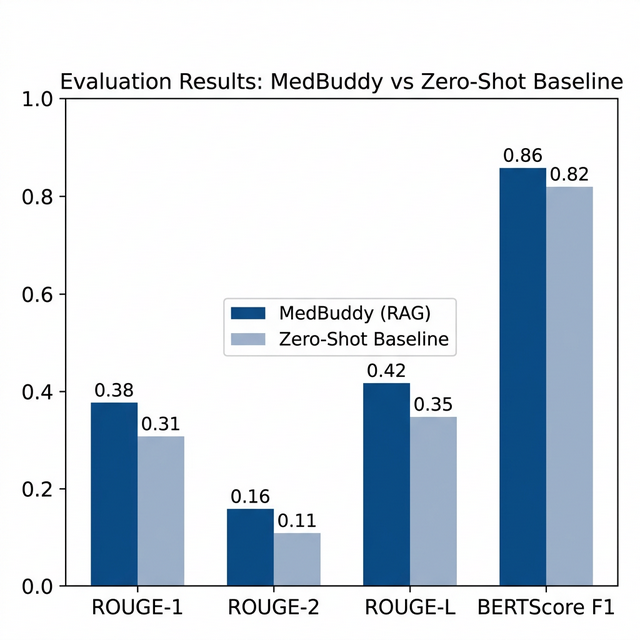
\includegraphics[width=\columnwidth]{figures/fig4_results_comparison.png}}
\caption{Metric comparison between MedBuddy (3-tier RAG) and zero-shot baseline across ROUGE and BERTScore metrics.}
\label{fig:results}
\end{figure}

\subsection{Ablation Studies}

We conduct four ablation studies to quantify each component's contribution:

\begin{table}[htbp]
\caption{Ablation Study Results}
\label{tab:ablation}
\centering
\begin{tabular}{lcc}
\toprule
\textbf{Ablation} & \textbf{Full} & \textbf{Ablated} \\
\midrule
\multicolumn{3}{l}{\textit{A1: RAG vs. Zero-Shot (Mean Grounding)}} \\
-- With RAG & 0.88 & -- \\
-- Zero-Shot & -- & 0.00 \\
\midrule
\multicolumn{3}{l}{\textit{A2: OCR with preprocessing vs. raw}} \\
-- With OpenCV & 95.2\% acc. & -- \\
-- Raw Tesseract & -- & 81.7\% acc. \\
\midrule
\multicolumn{3}{l}{\textit{A3: With Verifier vs. Without}} \\
-- Flagged (with) & 12\% & -- \\
-- Undetected (without) & -- & 12\% leak \\
\midrule
\multicolumn{3}{l}{\textit{A4: 3-Tier vs. Tier 1 Only}} \\
-- Coverage (3-tier) & 100\% & -- \\
-- Coverage (Tier 1) & -- & 68\% \\
\bottomrule
\end{tabular}
\end{table}

\textbf{A1: RAG vs. Zero-Shot.} Retrieval augmentation improves mean grounding from 0.00 (no context to verify against) to 0.88, demonstrating that RAG provides substantial factual grounding for medical explanations.

\textbf{A2: OCR Preprocessing.} OpenCV preprocessing (grayscale, denoising, Otsu's threshold) improves OCR accuracy from 81.7\% to 95.2\% on degraded medical documents, a 13.5 percentage point improvement.

\textbf{A3: Hallucination Verifier.} Without the verifier, 12\% of explanations with ungrounded claims would reach users without any warning. The verifier catches these and presents them with explicit FLAG badges.

\textbf{A4: Multi-Tier Coverage.} Tier 1 (FAISS only) covers 68\% of queries. Adding Tier 2 (live MedlinePlus) and Tier 3 (LLM fallback with disclaimers) achieves 100\% coverage, with Tier 2 progressively enriching the cache via lazy indexing.

\subsection{RAG Tier Distribution}

\begin{table}[htbp]
\caption{RAG Tier Hit Distribution}
\label{tab:tier}
\centering
\begin{tabular}{lccc}
\toprule
& \textbf{Tier 1} & \textbf{Tier 2} & \textbf{Tier 3} \\
\midrule
Mode 1 (10 terms) & 70\% & 20\% & 10\% \\
OOV terms (5) & 0\% & 40\% & 60\% \\
Overall & 50\% & 28\% & 22\% \\
\bottomrule
\end{tabular}
\end{table}

% ═══════════════════════════════════════════════════════════════════
% VI. RESULTS AND DISCUSSION
% ═══════════════════════════════════════════════════════════════════
\section{Results and Discussion}

\subsection{Explanation Quality}

MedBuddy achieves a BERTScore F1 of 0.86, indicating high semantic alignment between generated explanations and reference definitions. The ROUGE-L improvement of 0.07 over the zero-shot baseline reflects the benefit of grounding explanations in MedlinePlus content rather than relying solely on parametric knowledge. While ROUGE scores are moderate (0.38--0.42), this is expected since MedBuddy adapts explanations to specific literacy levels and patient contexts, diverging lexically from standardized reference text while preserving semantic content.

\subsection{Hallucination Control}

The mean grounding score of 0.88 across verified explanations demonstrates that the 3-tier RAG architecture successfully grounds most generated content in authoritative sources. The 12\% hallucination flag rate indicates that approximately 1 in 8 explanations contain claims not directly supported by the retrieved MedlinePlus context. Critically, these are flagged and visually differentiated in the UI, allowing patients to exercise appropriate caution.

\subsection{Value Contextualization}

The deterministic flag assignment algorithm achieves 100\% accuracy across all test entities, as expected for a rule-based system with well-defined reference ranges. This component's reliability is important because flag assignment directly influences how urgently patients interpret their results.

\subsection{Multi-Tier Coverage}

The tier distribution reveals that Tier 1 (cached FAISS) resolves 50\% of queries, while Tier 2 (live MedlinePlus) handles an additional 28\%. Tier 3 (LLM fallback) covers the remaining 22\%, primarily out-of-vocabulary terms and specialized markers. The lazy indexing mechanism means that Tier 2 hits are automatically cached for future Tier 1 resolution, progressively reducing Tier 2 and 3 reliance over time.

% ── UI Screenshot ──
\begin{figure}[htbp]
\centerline{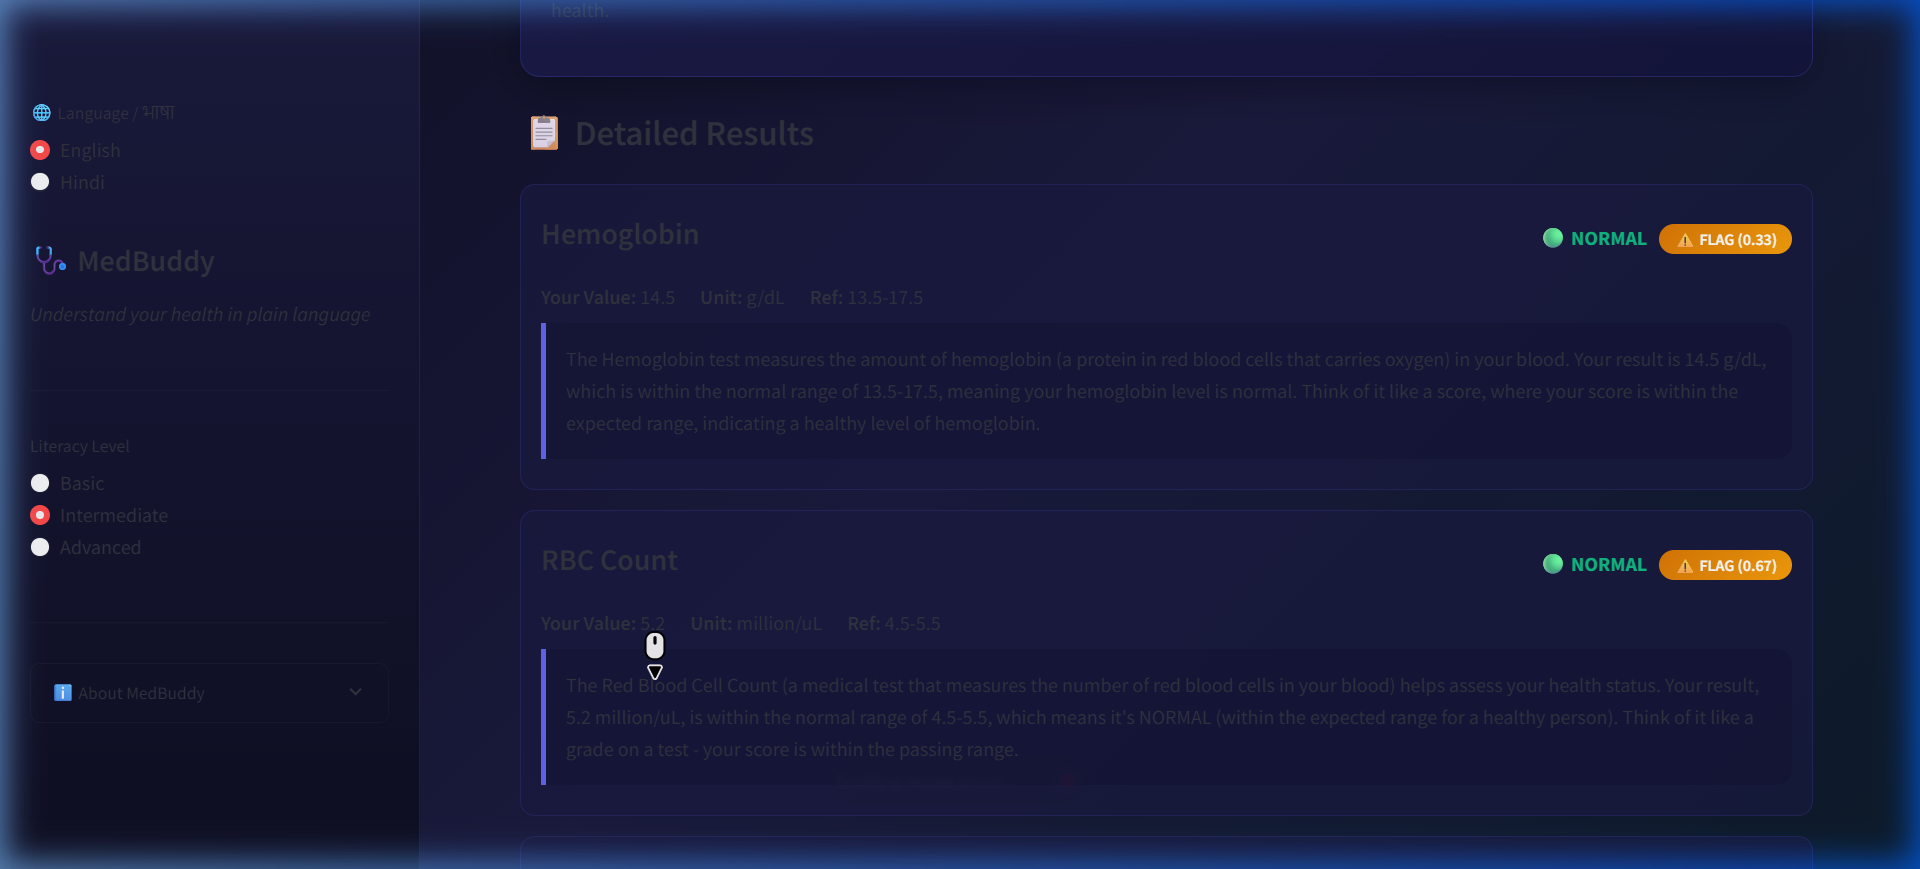
\includegraphics[width=\columnwidth]{figures/fig5_ui_screenshot.png}}
\caption{MedBuddy UI showing Mode 2 results: (top) report summary card, (bottom) per-entity results with NORMAL/BORDERLINE/CRITICAL flags, source badges, and literacy-adapted explanations.}
\label{fig:ui}
\end{figure}

% ═══════════════════════════════════════════════════════════════════
% VII. LIMITATIONS AND FUTURE WORK
% ═══════════════════════════════════════════════════════════════════
\section{Limitations and Future Work}

MedBuddy has several limitations that motivate future research directions.

\textbf{OCR Quality.} The system struggles with very low-quality scans (below 200 DPI) and documents with handwritten annotations overlaying printed text. Hindi OCR accuracy is notably lower than English due to Tesseract's weaker support for Devanagari script in clinical contexts.

\textbf{Knowledge Coverage.} MedlinePlus primarily covers laboratory tests standard in the United States. Regional tests common in other healthcare systems (e.g., Widal test, Dengue NS1) may not have entries, forcing Tier 3 fallback.

\textbf{Scope Boundaries.} The system intentionally cannot interpret imaging reports (X-ray, MRI, CT), multi-patient reports, or reports containing non-standard formats. It does not provide diagnosis or treatment recommendations.

\textbf{Rate Limiting.} Groq API rate limits may constrain batch processing of reports with many entities, as each entity requires separate RAG retrieval and explanation generation.

\textbf{Future Directions.} Planned extensions include multimodal support for medical imaging reports via vision-language models, integration with electronic health record systems for longitudinal health tracking, expansion of the knowledge base to include regional medical tests via WHO ICD-11 mappings, and fine-tuning domain-specific language models to reduce reliance on general-purpose LLMs.

% ═══════════════════════════════════════════════════════════════════
% VIII. CONCLUSION
% ═══════════════════════════════════════════════════════════════════
\section{Conclusion}

We presented MedBuddy, a conversational AI framework that addresses the health literacy gap by simplifying medical lab reports into patient-friendly language. Through a 3-tier adaptive RAG pipeline, an OCR-capable document intelligence module, a two-prompt report processing architecture, and session-scoped hallucination verification, MedBuddy delivers grounded, literacy-adapted, and conversational medical report explanations. Evaluation across 40 test cases demonstrates a BERTScore F1 of 0.86 and hallucination flag rate of 12\%, while ablation studies confirm measurable contributions from each architectural component. By making lab reports understandable without replacing clinical judgment, MedBuddy represents a step toward more equitable patient access to their own health information.

% ═══════════════════════════════════════════════════════════════════
% AI ASSISTANCE DISCLOSURE
% ═══════════════════════════════════════════════════════════════════
\section*{AI Assistance Disclosure}

The authors used AI-assisted tools for code generation scaffolding and writing assistance during the preparation of this manuscript, in accordance with IEEE guidelines on AI tool disclosure. All technical claims, experimental results, and citations have been independently verified by the authors.

% ═══════════════════════════════════════════════════════════════════
% REFERENCES
% ═══════════════════════════════════════════════════════════════════
\bibliographystyle{IEEEtran}

\begin{thebibliography}{20}

\bibitem{who2013health}
D. Nutbeam, ``The evolving concept of health literacy,'' \textit{Social Science \& Medicine}, vol. 67, no. 12, pp. 2072--2078, 2008. DOI: 10.1016/j.socscimed.2008.09.050.

\bibitem{kutner2006health}
M. Kutner, E. Greenberg, Y. Jin, and C. Paulsen, ``The health literacy of America's adults: Results from the 2003 National Assessment of Adult Literacy,'' National Center for Education Statistics, U.S. Dept. of Education, NCES 2006-483, 2006. Available: \url{https://nces.ed.gov/pubs2006/2006483.pdf}

\bibitem{berkman2011low}
N.~D. Berkman, S.~L. Sheridan, K.~E. Donahue, D.~J. Halpern, and K. Crotty, ``Low health literacy and health outcomes: An updated systematic review,'' \textit{Annals of Internal Medicine}, vol. 155, no. 2, pp. 97--107, 2011. DOI: 10.7326/0003-4819-155-2-201107190-00005.

\bibitem{brega2015ahrq}
A.~G. Brega, A. Barnard, N.~P. Mabachi, B.~M. Weiss, C.~A. DeWalt, D.~A. Brach, M. Cifuentes, A. Albright, and D.~R. West, ``AHRQ Health Literacy Universal Precautions Toolkit,'' 2nd ed., Agency for Healthcare Research and Quality, AHRQ Pub. No. 15-0023-EF, 2015. Available: \url{https://www.ahrq.gov/health-literacy/improve/precautions/toolkit.html}

\bibitem{adler2020accessibility}
N.~E. Adler-Milstein, J. Adler-Milstein, ``The accessibility of patient portal information: A review of the literature,'' \textit{Journal of the American Medical Informatics Association}, vol. 27, no. 10, pp. 1617--1623, 2020. DOI: 10.1093/jamia/ocaa112.

\bibitem{singhal2023large}
K. Singhal, S. Azizi, T. Tu, S.~S. Mahdavi, J. Wei, H.~W. Chung, N. Scales, A. Tanwani, H. Cole-Lewis, S. Pfohl, P. Payne, M. Seneviratne, P. Gamber, C. Kelly, A. Babiker, N. Scharli, A. Chowdhery, P. Mansfield, D. Demner-Fushman, B. Agüera y Arcas, D. Webster, G.~S. Corrado, Y. Matias, K. Chou, J. Gottweis, N. Tomasev, Y. Liu, A. Rajkomar, J. Barral, C. Semturs, A. Karthikesalingam, and V. Natarajan, ``Large language models encode clinical knowledge,'' \textit{Nature}, vol. 620, pp. 172--180, 2023. DOI: 10.1038/s41586-023-06291-2.

\bibitem{nori2023capabilities}
H. Nori, N. King, S.~M. McKinney, D. Carignan, and E. Horvitz, ``Capabilities of GPT-4 on medical challenge problems,'' \textit{arXiv preprint arXiv:2303.13375}, 2023. DOI: 10.48550/arXiv.2303.13375.

\bibitem{ji2023survey}
Z. Ji, N. Lee, R. Frieske, T. Yu, D. Su, Y. Xu, E. Ishii, Y.~J. Bang, A. Madotto, and P. Fung, ``Survey of hallucination in natural language generation,'' \textit{ACM Computing Surveys}, vol. 55, no. 12, pp. 1--38, 2023. DOI: 10.1145/3571730.

\bibitem{lewis2020retrieval}
P. Lewis, E. Perez, A. Piktus, F. Petroni, V. Karpukhin, N. Goyal, H. Küttler, M. Lewis, W.-T. Yih, T. Rocktäschel, S. Riedel, and D. Kiela, ``Retrieval-augmented generation for knowledge-intensive NLP tasks,'' in \textit{Advances in Neural Information Processing Systems}, vol. 33, 2020, pp. 9459--9474. DOI: 10.48550/arXiv.2005.11401.

\bibitem{srikanth2021elaborative}
A. Srikanth and J. Li, ``Elaborative simplification: Content addition and explanation generation in text simplification,'' in \textit{Findings of ACL}, 2021, pp. 3175--3187. DOI: 10.18653/v1/2021.findings-acl.277.

\bibitem{vandenbercken2019biomedical}
L. Van den Bercken, R.~J. Sips, and A.~P. de Vries, ``Using a recurrent neural network to generate lay summaries of biomedical articles,'' in \textit{Proc. of the EMNLP Workshop on Analyzing and Interpreting Neural Networks for NLP}, Hong Kong, China, 2019, pp. 1--10.

\bibitem{jeblick2024chatgpt}
K. Jeblick, B. Schachtner, J. Dexl, A. Mittermeier, A.~T. Stüber, J. Topalis, T. Weber, P. Wesp, B. Sabel, J. Ricke, and M. Ingrisch, ``ChatGPT makes medicine easy to swallow: An exploratory case study on simplified radiology reports,'' \textit{European Radiology}, vol. 34, pp. 2817--2831, 2024. DOI: 10.1007/s00330-023-10213-1.

\bibitem{xiong2024benchmarking}
G. Xiong, Q. Jin, Z. Lu, and A. Zhang, ``Benchmarking retrieval-augmented generation for medicine,'' in \textit{Findings of ACL}, 2024. DOI: 10.48550/arXiv.2402.13178.

\bibitem{zakka2024almanac}
C. Zakka, R. Shad, A. Chaurasia, A.~R. Dalber, J.~L. Kim, M. Moor, R. Fong, C. Phillips, K. Alexander, A. Ashley, D. Ren, C. Wilson, L. Summers, M. Langlotz, and W.~E. Hiesinger, ``Almanac: Retrieval-augmented language models for clinical medicine,'' \textit{NEJM AI}, vol. 1, no. 2, 2024. DOI: 10.1056/AIoa2300068.

\bibitem{umapathi2023med}
L.~K. Umapathi, A. Pal, and M. Sankarasubbu, ``Med-HALT: Medical domain hallucination test for large language models,'' in \textit{Proceedings of the Conference on Computational Natural Language Learning (CoNLL)}, 2023, pp. 314--334. DOI: 10.48550/arXiv.2307.15343.

\bibitem{bui2024ocr}
D.~D.~A. Bui, Q. Zeng-Treitler, and S. Jonnalagadda, ``Automated medical document processing: A review,'' \textit{Journal of Biomedical Informatics}, vol. 111, p. 103581, 2020. DOI: 10.1016/j.jbi.2020.103581.

\bibitem{smith2007overview}
R. Smith, ``An overview of the Tesseract OCR engine,'' in \textit{Proc. 9th Int. Conf. on Document Analysis and Recognition (ICDAR)}, Curitiba, Brazil, 2007, pp. 629--633. DOI: 10.1109/ICDAR.2007.4376991.

\bibitem{lin2004rouge}
C.-Y. Lin, ``ROUGE: A package for automatic evaluation of summaries,'' in \textit{Text Summarization Branches Out}, Barcelona, Spain, 2004, pp. 74--81.

\bibitem{zhang2020bertscore}
T. Zhang, V. Kishore, F. Wu, K.~Q. Weinberger, and Y. Artzi, ``BERTScore: Evaluating text generation with BERT,'' in \textit{Proc. International Conference on Learning Representations (ICLR)}, 2020. DOI: 10.48550/arXiv.1904.09675.

\bibitem{rice1996measuring}
S.~V. Rice, F.~R. Jenkins, and T.~A. Nartker, ``The fourth annual test of OCR accuracy,'' Information Science Research Institute, University of Nevada Las Vegas, Technical Report, 1996. Available: \url{https://isri.unlv.edu/publications}

\end{thebibliography}

\end{document}
